\documentclass[aps,reprint,superscriptaddress,10pt]{revtex4-2}
\usepackage{kotex}
\usepackage[HWP]{dhucs-interword}
\usepackage[dvips]{color}
\usepackage{graphicx}
\usepackage{bm}
\usepackage{amsmath}
\usepackage{tikz}
\usepackage{natbib}
\usepackage{mhchem}
\usepackage{booktabs}
\usepackage{multirow}
\usepackage{array}
\usepackage{setspace}
\setstretch{1.4}



\begin{document}
\title{응집물질물리실험 결과보고서 \\
\small 실험주제 : Crystal Growth \& X-ray diffraction,
Structure transition of BaTiO3}

\author{HuiJae-Lee}\email{hjlee6674@inha.edu}
\affiliation{Physics Department, Inha University}

\date{\today}

\begin{abstract}
  X-ray diffraction을 이용하여 각 시료의 격자 상수를 구하고 격자 구조를 추정하였다. 또한
  온도에 따른 BaTiO$_3$의 캐퍼시턴스 $C_p$와 전기변위장 $D$의 크기를 관측하여
  BaTiO$_3$의 상전이 온도를 구하였다.
\end{abstract}

\maketitle

\section{Process}
\subsection{X-ray Diffraction}
\begin{itemize}
  \item[1. ] Ba, Sr, Ca를 각자 다른 사발에 넣고 모든 사발에 TiO$_3$를 몰 수에 맞춰 넣은 후
  30분 가량 동안 갈아준다. 
  \item[2. ] 충분히 갈아진 시료들을 캡슐에 담아 퍼니스에 넣어 $800~\mathrm{^\circ C}$ 이상의
  온도로 24시간 이상 가열한다.
  \item[3. ] 위의 과정을 3번 반복하여 최대한 많은 물질을 반응시킨다.
  \item[4. ] 반응시킨 시료를 인하대학교 표준분석연구원에 의뢰하여  X-ray Diffraction 
  데이터를 얻는다.
\end{itemize}

\subsection{Structure Transition of BaTiO$_3$}
\begin{itemize}
  \item[1. ] 준비된 기기에 온도계와 RLC미터를 연결한다.
  \item[2. ] 준비된 기기를 핫플레이트에 올려 가열시킬 준비를 한다.
  \item[3. ] 온도에 따른 커패시턴스와 전기변위장의 변화를 측정한다.
\end{itemize}
\section{Result}
\subsection{X-ray Diffraction}
X-ray diffraction은 본교 표준분석연구원에 의뢰를 맡겨 진행하였으며
사용된 X-ray의 파장은 1.54~$\mathrm{\AA}$이다.
%-----------------------------------------------------------------------------------------
%-----------------------------------------------------------------------------------------
%-----------------------------------------------------------------------------------------
\vspace{-1.2cm}
\subsubsection{CaTiO$_3$}
\begin{figure}[h!tb]
  \centering
  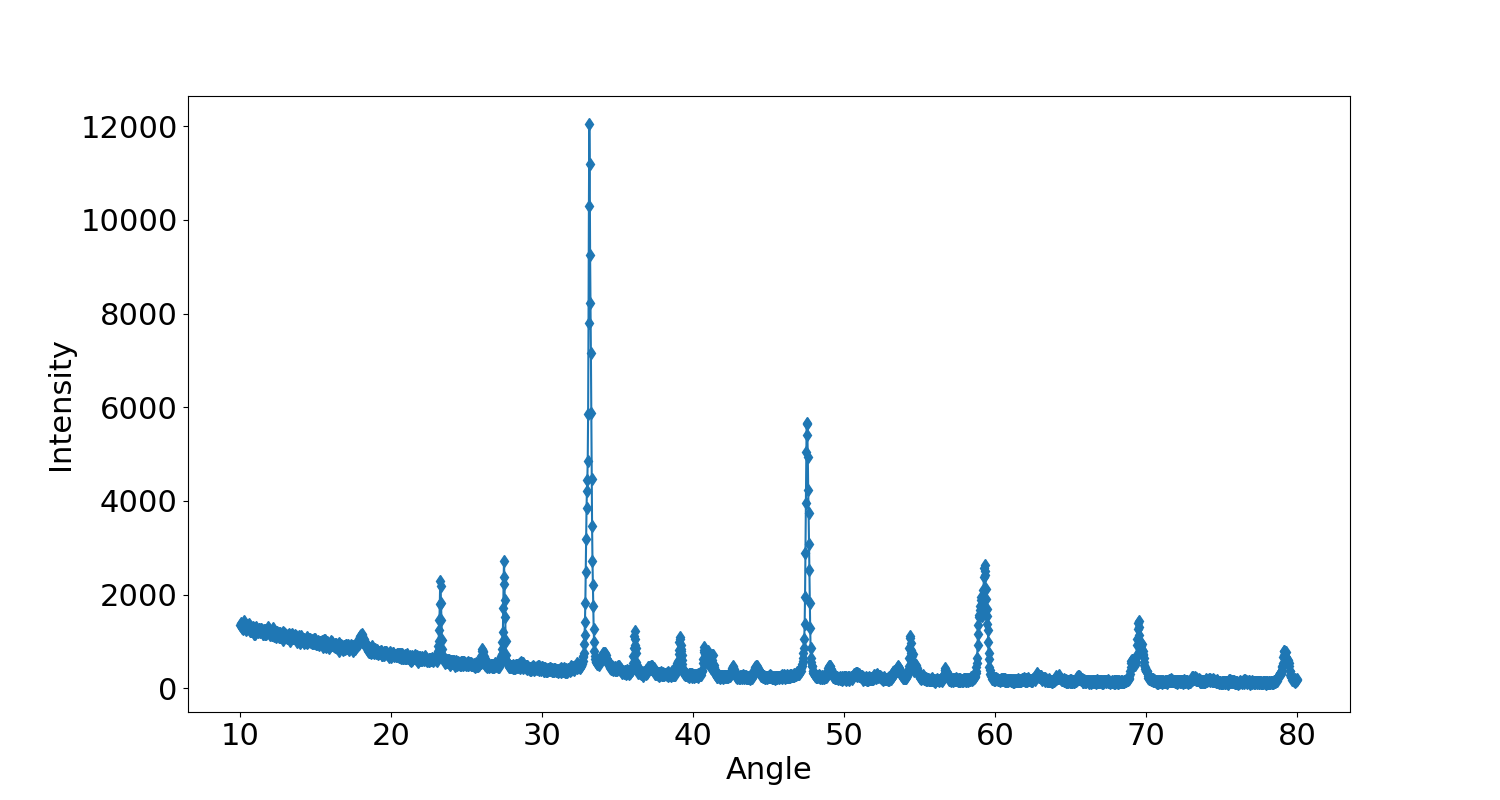
\includegraphics[scale=0.16]{Ca.png}
  \caption{CaTiO$_3$의 XRD 패턴}
  \label{fig:Ca}
\end{figure}
\vspace{-1.2cm}
%-----------------------------------------------------------------------------------------
%-----------------------------------------------------------------------------------------
%-----------------------------------------------------------------------------------------
\subsubsection{SrTiO$_3$}
\begin{figure}[h!tb]
  \centering
  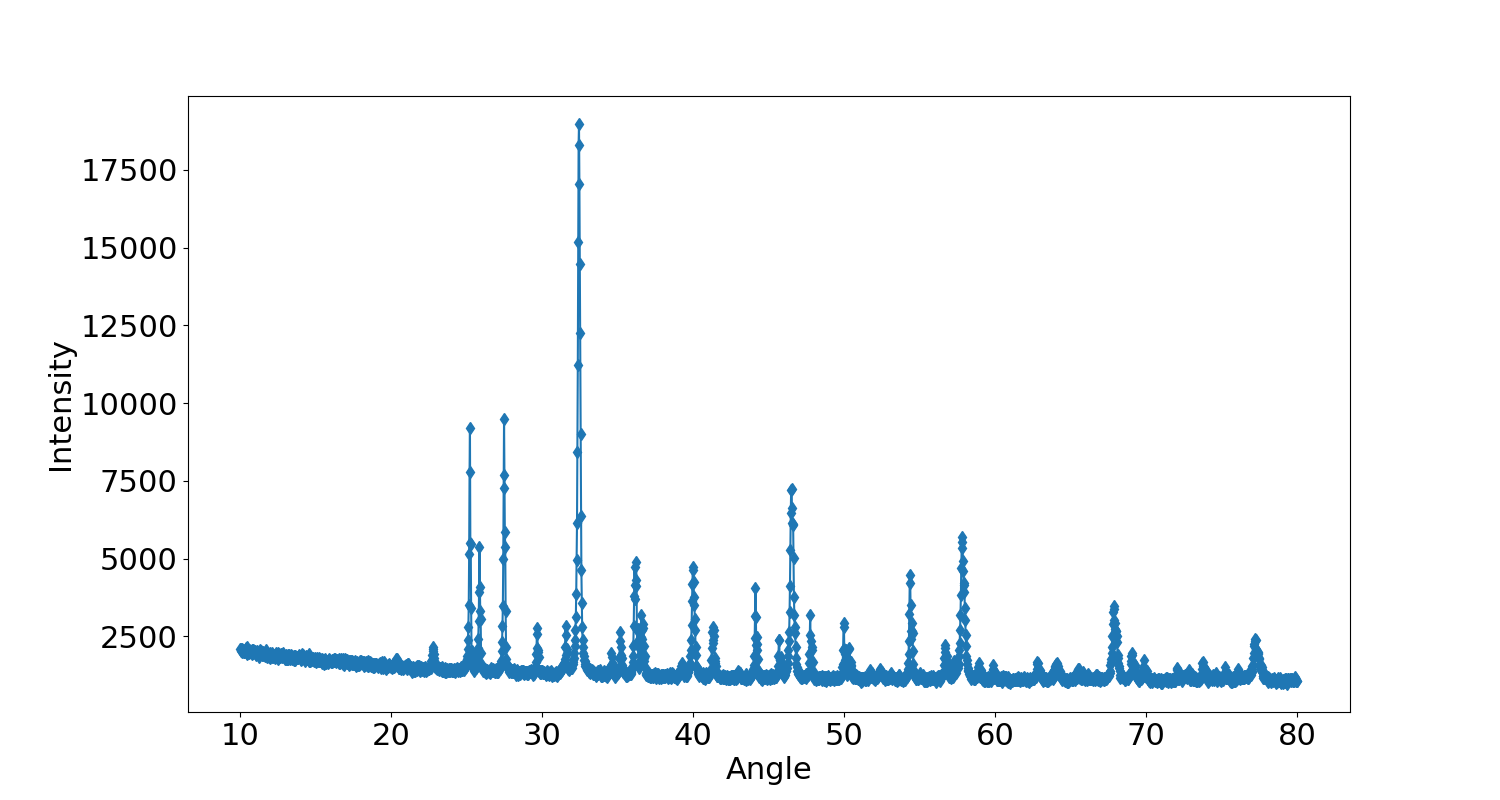
\includegraphics[scale=0.16]{Sr.png}
  \caption{SrTiO$_3$의 XRD 패턴}
  \label{fig:Sr}
\end{figure}
%-----------------------------------------------------------------------------------------
%-----------------------------------------------------------------------------------------
%-----------------------------------------------------------------------------------------
\vspace{-1.2cm}
\subsubsection{BaTiO$_3$}
  \begin{figure}[h!tb]
    \centering
    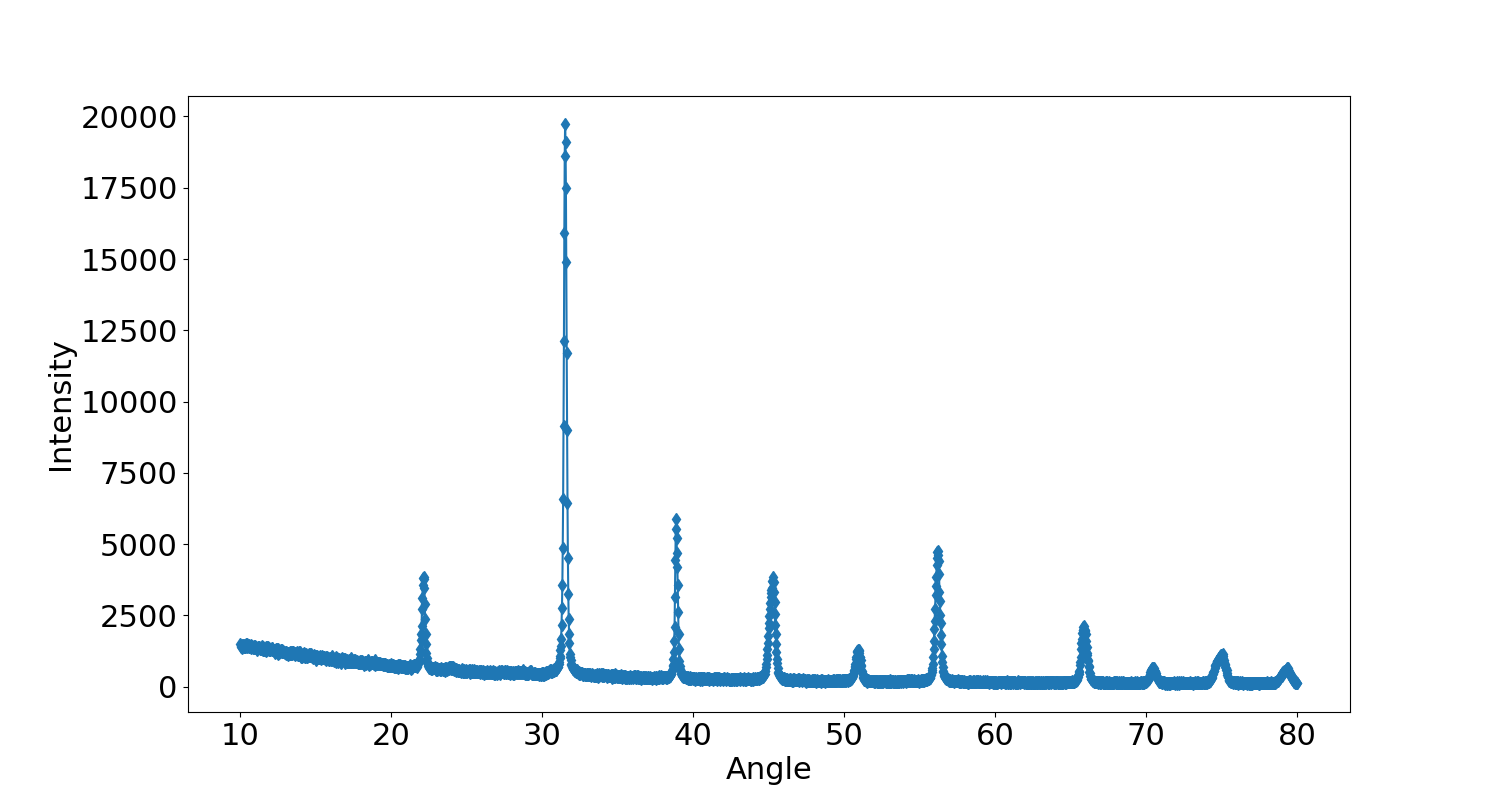
\includegraphics[scale=0.16]{Ba.png}
    \caption{BaTiO$_3$의 XRD 패턴}
    \label{fig:Ba}
    \end{figure}
%----------------------------------------------------------------------------------------
%-----------------------------------------------------------------------------------------
%-----------------------------------------------------------------------------------------
\newpage
\subsection{Structure Transition of BaTiO$_3$}
\begin{figure}[htb!]
  \centering
  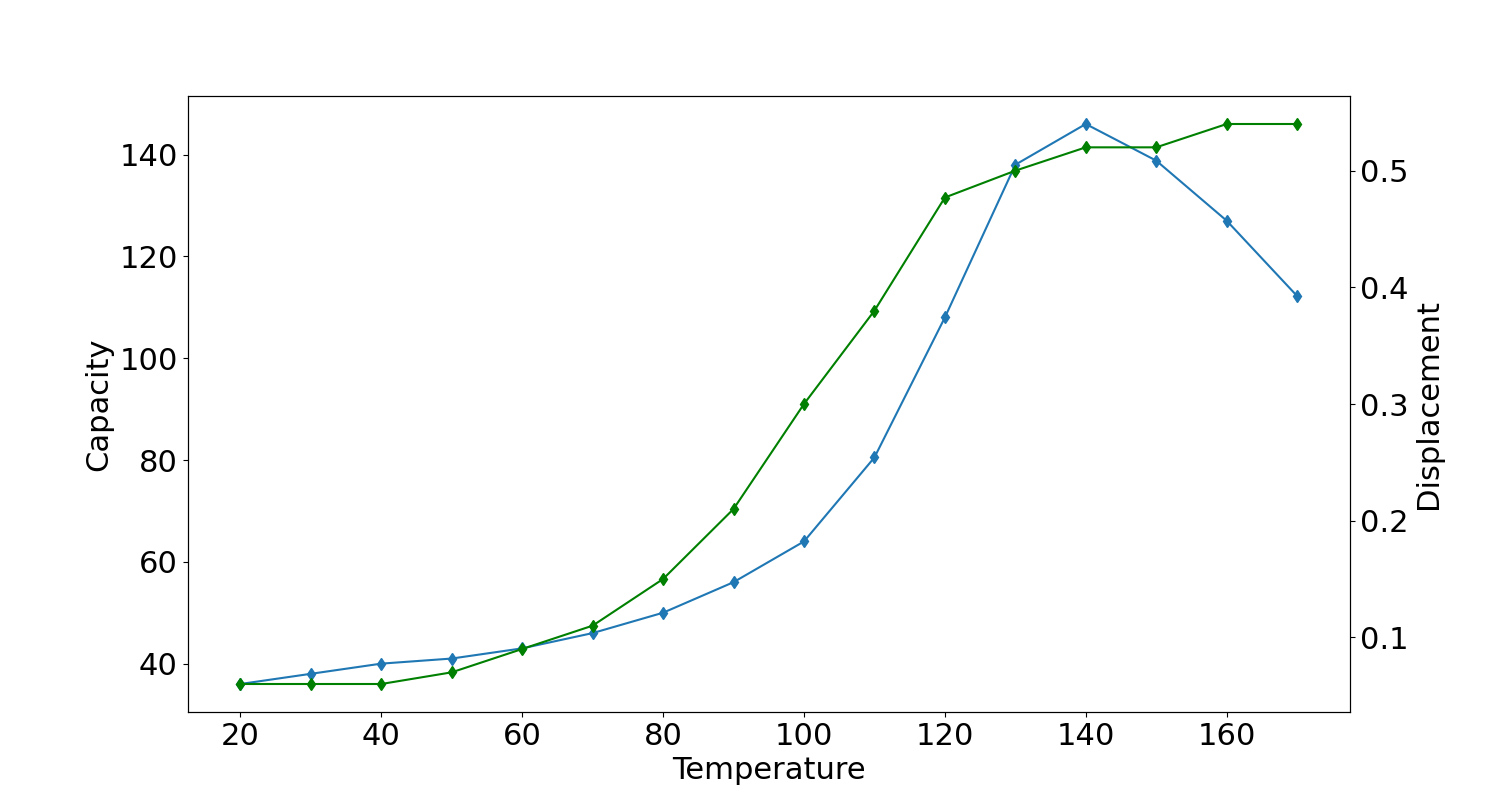
\includegraphics[scale=0.2]{CD.png}
  \caption{BaTiO$_3$의 온도에 따른 상전이에 의한 $C_p$와 $D$의 변화}
  \label{fig:CD}
\end{figure}

BaTiO$_3$의 상전이 온도를 구하기 위해 해당 시료에 양 극판을 붙인 축전기에 전압을 인가하여
BaTiO$_3$의 캐퍼시턴스 $C_p$와 전기변위장 $D$의 크기를 관측한 결과,
전기변위장 $D$는 온도가 증가함에 따라 계속 증가하였지만
캐퍼시턴스 $C_p$는 140~$^\circ$C에서 최댓값을 가지고 온도가 증가함에 따라 감소하는 결과를
얻었다.
%-----------------------------------------------------------------------------------------
%-----------------------------------------------------------------------------------------
%-----------------------------------------------------------------------------------------
%-----------------------------------------------------------------------------------------
%-----------------------------------------------------------------------------------------
%-----------------------------------------------------------------------------------------


\section{Analysis}
\subsection{X-ray Diffraction}
X-ray diffraction의 이론적인 값으로부터 각 물질의 격자 상수를 계산할 수 있다.
FIG~\ref{fig:Ca1}, FIG~\ref{fig:Sr1}, FIG~\ref{fig:Ba1}의 peak 위에 기입된
세개의 숫자는 Miller index로 격자 상수를 계산하는데 쓰인다. Miller index가 
$h,k,l$로 주어졌다면 Bragg 법칙과 면간 거리 $d$에 대한 식을 다음과 같이 쓸 수 있다.
\begin{align}
  \label{eq:1} d_{hkl} &= \frac{\lambda}{2\sin\theta},\,\,\,  \\
  \label{eq:2} \frac{1}{d_{hkl}^2} &=\left(\frac{h}{a}\right)^2
  +\left(\frac{k}{b}\right)^2+\left(\frac{l}{c}\right)^2.
\end{align}
a, b, c는 격자 상수이다.
%-----------------------------------------------------------------------------------------
%-----------------------------------------------------------------------------------------
%-----------------------------------------------------------------------------------------
\newpage
\subsubsection{CaTiO$_3$}
\vspace{-0.5cm}
\begin{figure}[htb!]
  \centering
  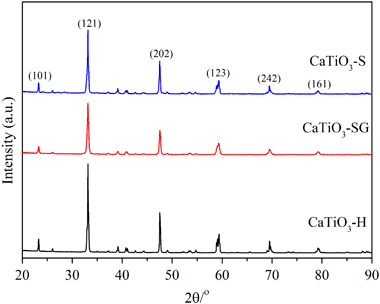
\includegraphics[scale=0.45]{Ca1.png}
  \caption{CaTiO$_3$의 이론 상 XRD 패턴}
  \label{fig:Ca1}
\end{figure}
\begin{table}[htp]
  \centering
  \begin{tabular}{>{\centering}p{0.12\textwidth}
    >{\centering}p{0.12\textwidth}
    >{\centering\arraybackslash}p{0.12\textwidth}}
      \toprule
      Miller index& Angle($^\circ$) & Intensity \\
      \midrule
      (101)&23.24 &2285 \\
      (121)&33.11 &12048 \\
      (202)&47.50 &5664 \\
      (123)&59.29 &2638\\
      (242)&69.48 &1445\\
      (161)&79.13 &798 \\
      \bottomrule
  \end{tabular}
  \caption{FIG.~\ref{fig:Ca1}에서 볼 수 있는 Miller index와 그 angle에 따른
  FIG.~\ref{fig:Ca}에서의 intensity. }\label{table:1}
\end{table}

Peak가 확실하게 보이는 (121), (202), (123)을 택하여 식~\eqref{eq:1}을 이용해 
$d_{hkl}$를 구하면 다음과 같다(TABLE~\ref{table:1-1}).

\begin{table}[htp]
  \centering
  \begin{tabular}{>{\centering}p{0.12\textwidth}
    >{\centering\arraybackslash}p{0.12\textwidth}}
      \toprule
      $d_{hkl}$& Value($\mathrm{\AA}$) \\
      \midrule
      $d_{121}$&1.410 \\
      $d_{202}$&1.044 \\
      $d_{123}$&0.8956 \\
      \bottomrule
  \end{tabular}
  \caption{CaTiO$_3$의 $d_{hkl}$.}\label{table:1-1}
\end{table}

이 값을 식~\eqref{eq:2}에 대입하여 격자 상수 $a,b,c$를 구할 수 있다(TABLE~\ref{table:1-2}).
\begin{table}[h!tp]
  \centering
  \begin{tabular}{>{\centering}p{0.12\textwidth}
    >{\centering\arraybackslash}p{0.12\textwidth}}
      \toprule
      $a,b,c$& Value \\
      \midrule
      $a$&5.42872\\
      $b$&7.6394\\
      $c$&5.3867\\
      \bottomrule
  \end{tabular}
  \caption{CaTiO$_3$의 격자 상수 $a,b,c$.}\label{table:1-2}
\end{table}
%-----------------------------------------------------------------------------------------
%-----------------------------------------------------------------------------------------
%-----------------------------------------------------------------------------------------
\newpage
\subsubsection{SrTiO$_3$}
\vspace{-0.5cm}
\begin{figure}[htb!]
  \centering
  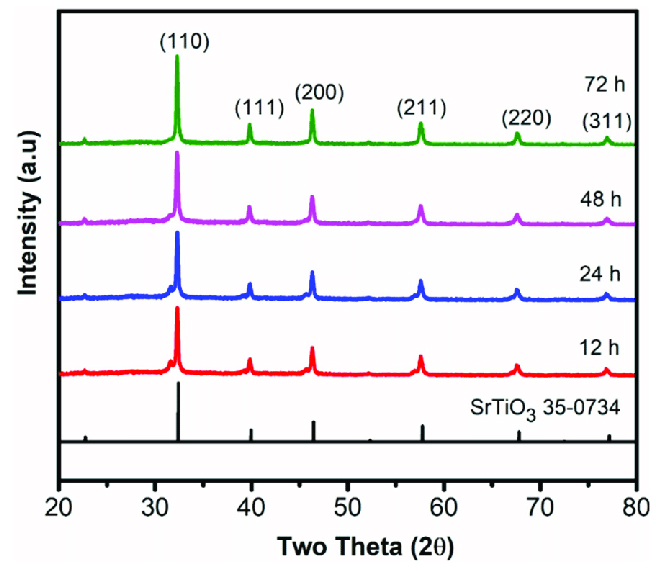
\includegraphics[scale=0.3]{Sr1.png}
  \caption{SrTiO$_3$의 이론 상 XRD 패턴}
  \label{fig:Sr1}
\end{figure}
\begin{table}[htp]
  \centering
  \begin{tabular}{>{\centering}p{0.12\textwidth}
    >{\centering}p{0.12\textwidth}
    >{\centering\arraybackslash}p{0.12\textwidth}}      \toprule
      Miller index & Angle($^\circ$) & Intensity \\
      \midrule
      (110)& 32.43 &18974 \\
      (111)& 39.97 &4729 \\
      (200)& 46.50 &7229 \\
      (211)& 57.79 &5705 \\
      (220)& 67.83 &3477 \\
      (311)& 77.23 &2379 \\
      \bottomrule
  \end{tabular}
  \caption{FIG.~\ref{fig:Sr1}에서 볼 수 있는 Miller index와 그 angle에 따른
  FIG.~\ref{fig:Sr}에서의 intensity. }\label{table:2}
\end{table}

Peak가 확실하게 보이는 (110), (111), (200)을 택하여 식~\eqref{eq:1}을 이용해 
$d_{hkl}$를 구하면 다음과 같다(TABLE~\ref{table:2-1}).

\begin{table}[htb!]
  \centering
  \begin{tabular}{>{\centering}p{0.12\textwidth}
    >{\centering\arraybackslash}p{0.12\textwidth}}
      \toprule
      $d_{hkl}$& Value($\mathrm{\AA}$) \\
      \midrule
      $d_{110}$&1.410 \\
      $d_{111}$&1.044 \\
      $d_{200}$&0.8956 \\
      \bottomrule
  \end{tabular}
  \caption{SrTiO$_3$의 $d_{hkl}$.}\label{table:2-1}
\end{table}

이 값을 식~\eqref{eq:2}에 대입하여 격자 상수 $a,b,c$를 구할 수 있다(TABLE~\ref{table:2-2}).

\begin{table}[htb!]
  \centering
  \begin{tabular}{>{\centering}p{0.12\textwidth}
    >{\centering\arraybackslash}p{0.12\textwidth}}
      \toprule
      $a,b,c$& Value \\
      \midrule
      $a$&3.90126\\
      $b$&3.89801\\
      $c$&3.90741\\
      \bottomrule
  \end{tabular}
  \caption{SrTiO$_3$의 격자 상수 $a,b,c$.}\label{table:2-2}
\end{table}
%-----------------------------------------------------------------------------------------
%-----------------------------------------------------------------------------------------
%-----------------------------------------------------------------------------------------

\subsubsection{BaTiO$_3$}
\vspace{-0.3cm}
\begin{figure}[ht]
  \centering
  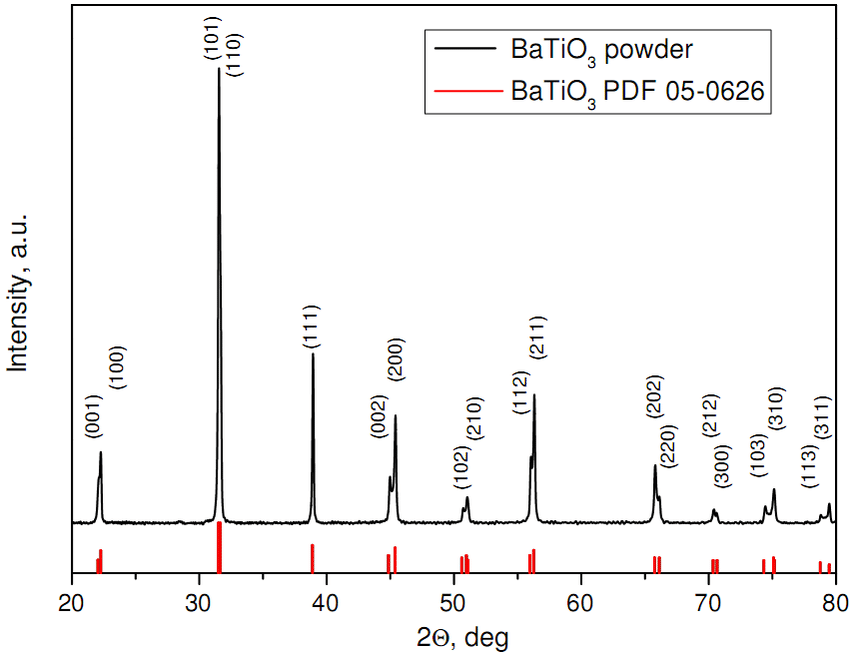
\includegraphics[scale=0.25]{Ba1.png}
  \caption{BaTiO$_3$의 이론 상 XRD 패턴}
  \label{fig:Ba1}
\end{figure}


  \begin{table}[ht]
    \centering
    \begin{tabular}{>{\centering}p{0.12\textwidth}
      >{\centering}p{0.12\textwidth}
      >{\centering\arraybackslash}p{0.12\textwidth}} 
      \toprule
      Miller index & Angle($^\circ$) & Intensity \\
      \midrule
      (100)& 22.13 &3865 \\
      (101)& 31.51 &19735 \\
      (111)& 38.86 &5886 \\
      (200)& 45.22 &3701 \\
      (210)& 50.89 &1303 \\
      (211)& 56.19 &4752 \\
      (202)& 65.88 &2130 \\
      (212)& 70.40 &665 \\
      (310)& 75.05 &1164 \\
      (311)& 79.38 &661 \\
      \bottomrule
  \end{tabular}
  \caption{FIG.~\ref{fig:Ba1}에서 볼 수 있는 Miller index와 그 angle에 따른
  FIG.~\ref{fig:Ba}에서의 intensity. }\label{table:3}
\end{table}

Peak가 확실하게 보이는 (100), (101), (111)을 택하여 식~\eqref{eq:1}을 이용해 
$d_{hkl}$를 구하면 다음과 같다(TABLE~\ref{table:3-1}).



\begin{table}[ht]
  \centering
  \begin{tabular}{>{\centering}p{0.12\textwidth}
    >{\centering\arraybackslash}p{0.12\textwidth}}
      \toprule
      $d_{hkl}$& Value($\mathrm{\AA}$) \\
      \midrule
      $d_{100}$&1.410 \\
      $d_{101}$&1.044 \\
      $d_{111}$&0.8956 \\
      \bottomrule
  \end{tabular}
  \caption{BaTiO$_3$의 $d_{hkl}$.}\label{table:3-1}
\end{table}

이 값을 식~\eqref{eq:2}에 대입하여 격자 상수 $a,b,c$를 구할 수 있다(TABLE~\ref{table:3-2}).

\begin{table}[ht]
  \centering
  \begin{tabular}{>{\centering}p{0.12\textwidth}
    >{\centering\arraybackslash}p{0.12\textwidth}}
      \toprule
      $a,b,c$& Value \\
      \midrule
      $a$&4.01204\\
      $b$&4.00663\\
      $c$&4.00893\\
      \bottomrule
  \end{tabular}
  \caption{BaTiO$_3$의 격자 상수 $a,b,c$.}\label{table:3-2}
\end{table}

\newpage
X-ray diffracion으로 알아낸 각 시료의 격자 상수와 각 시료의 이론적 격자 상수를
비교하여 각 시료의 구조를 알아낼 수 있다. 격자 상수의 오차는 다음과 
같다(TABLE~\ref{table:result}).

\begin{table}[ht]
  \centering
  \begin{tabular}{>{\centering}p{0.12\textwidth}
    >{\centering}p{0.12\textwidth}
    >{\centering\arraybackslash}p{0.12\textwidth}} 
    \toprule
    $a,b,c$(CaTiO$_3$) & 이론값 & 상대오차(\%) \\
    \midrule
    $a$& 5.51 & 1.48 \\
    $b$& 7.69 & 0.658 \\
    $c$& 5.41 & 0.431 \\
    \bottomrule
\end{tabular}

\begin{tabular}{>{\centering}p{0.12\textwidth}
  >{\centering}p{0.12\textwidth}
  >{\centering\arraybackslash}p{0.12\textwidth}} 
  \toprule
  $a,b,c$(SrTiO$_3$) & 이론값 & 상대오차(\%) \\
  \midrule
  $a$& 3.95 & 1.23 \\
  $b$& 3.95 & 1.32 \\
  $c$& 3.95 & 1.08 \\
  \bottomrule
\end{tabular}

\begin{tabular}{>{\centering}p{0.12\textwidth}
  >{\centering}p{0.12\textwidth}
  >{\centering\arraybackslash}p{0.12\textwidth}} 
  \toprule
  $a,b,c$(BaTiO$_3$) & 이론값 & 상대오차(\%) \\
  \midrule
  $a$& 4.20 & 4.48 \\
  $b$& 4.00 & -0.166 \\
  $c$& 4.00 & -0.223 \\
  \bottomrule
\end{tabular}
\caption{CaTiO$_3$, SrTiO$_3$, BaTiO$_3$의 격자 상수 $a,b,c$의
이론값과 상대오차.}\label{table:result}
\end{table}
이로 부터 각 시료의 구조를 알 수 있는데 CaTiO$_3$는 orthorhombic,
SrTiO$_3$는 cubic, BaTiO$_3$는 tetragonal이다.


%-----------------------------------------------------------------------------------------
%-----------------------------------------------------------------------------------------
%-----------------------------------------------------------------------------------------

\subsection{Structure Transition of BaTiO$_3$}

\begin{figure}[h!]
  \centering
  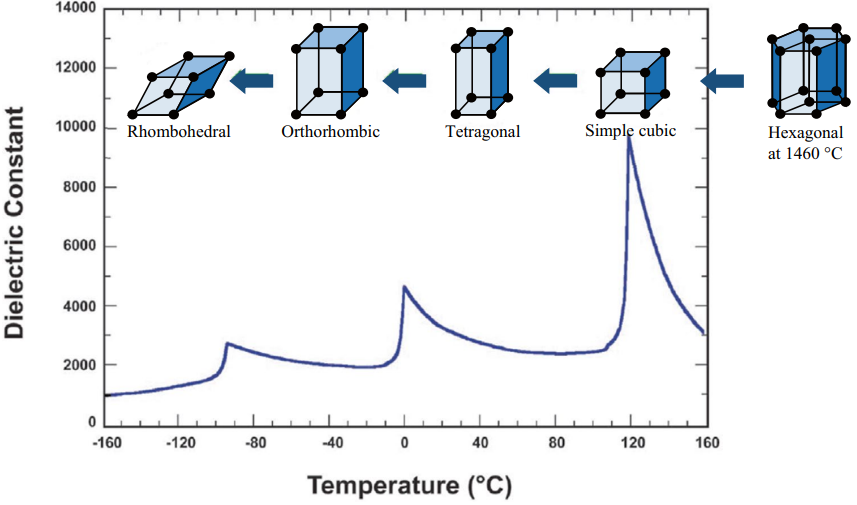
\includegraphics[scale=0.2]{capa.png}
  \caption{BaTiO$_3$의 온도에 따른 상전이에 의한 유전 상수의 변화}
  \label{fig:capa}
\end{figure}
BaTiO$_3$의 캐퍼시턴스 $C_p$는 평행판 축전기 사이에 위치해 있으므로 다음과 같은 관계에 있다.
\begin{align}
  C_p = \epsilon_0 \epsilon_r\frac{A}{d}.
\end{align}
$A$와 $d$는 각각 평행판의 넓이와 평행판 사이 거리이고 $\epsilon_0$와 $\epsilon_r$는
진공 유전율과 BaTiO$_3$의 유전율이다.
또한 전기변위장 $D$는
\begin{align}
  D = \epsilon_r E = \epsilon_r Vd
\end{align}
의 관계에 있다. $V$는 축전기의 양 극판에 걸리는 전압이다. 이 실험에서 평행판의 넓이 $A$와
전압 $V$는 상수이고 상전이로 인해 변할 수 있는 값은 BaTiO$_3$의 유전율 $\epsilon_r$과
평행판 사이 거리 $d$이다. BaTiO$_3$의 상전이로 인한 $d$의 변화가 무시할 수 있을 만큼 작다고
가정하면, BaTiO$_3$의 유전율 $\epsilon_r$의 변화는 $C_p$와 같고 이는 120~$^\circ$C 근처에서
상전이하는 BaTiO$_3$의 특성보다 약 20~$^\circ$C의 차이를 보인다.

\section{Conclusion}
\subsection{X-ray Diffraction}
\begin{itemize}
  \item[1. ] X-ray diffraction을 이용하여 구한 격자 상수의 상대 오차가 모두 5\% 이내인
  점으로부터, CaTiO$_3$는 orthorhombic, SrTiO$_3$는 cubic, BaTiO$_3$는 tetragonal의 
  구조를 이루고 있다는 결론은 타당하다고 판단할 수 있다.
  \item[2. ] 직접 측정한 SrTiO$_3$의 XRD 패턴이 이론적인 패턴보다 더 많은 peak를 가지는데
  실험을 진행하는 과정에서 불순물이 첨가된 것으로 보인다. 시료를 막자 사발에 가는 과정에서
  막자 사발의 일부가 깨진 적이 있는데 SrTiO$_3$의 이론적인 XRD 패턴과 불일치 하는 peak 중
  SiO$_2$의 peak 부분인 23$^\circ$에서 높은 intensity가 관측된 것을 보아 막자 사발의 일부가
  시료에 들어가 같이 관측된 것이라 추측한다.

\end{itemize}
\subsection{Structure Transition of BaTiO$_3$}
\begin{itemize}
  \item[1. ] BaTiO$_3$의 상전이 온도를 측정하는 실험에서 실험으로 추정한 140~$^\circ$C와
  이론값인 약 120~$^\circ$C가 약 20~$^\circ$C의 차이를 보였는데 실제로 온도를 측정한 실리콘
  액체와 BaTiO$_3$ 사이의 온도차로 인한 오차라고 생각한다.
  \item[2. ] 온도를 140~$^\circ$C 보다 높이는 도중에 축전기에 silver epoxy로 연결된 도선이
  분리되어 실험을 중단할 수 밖에 없었는데 더 높은 온도에서 $C_p$와 $D$의 변화를 측정하지 못한
  점이 아쉬움으로 남는다.
\end{itemize}
\nocite{*}
\bibliography{ref}



%\begin{thebibliography}{9}
%\end{thebibliography}

\vfill
\end{document}